\chapter{Diagramme de séquence}

\section{Diagramme}

\begin{figure}
  \centering
  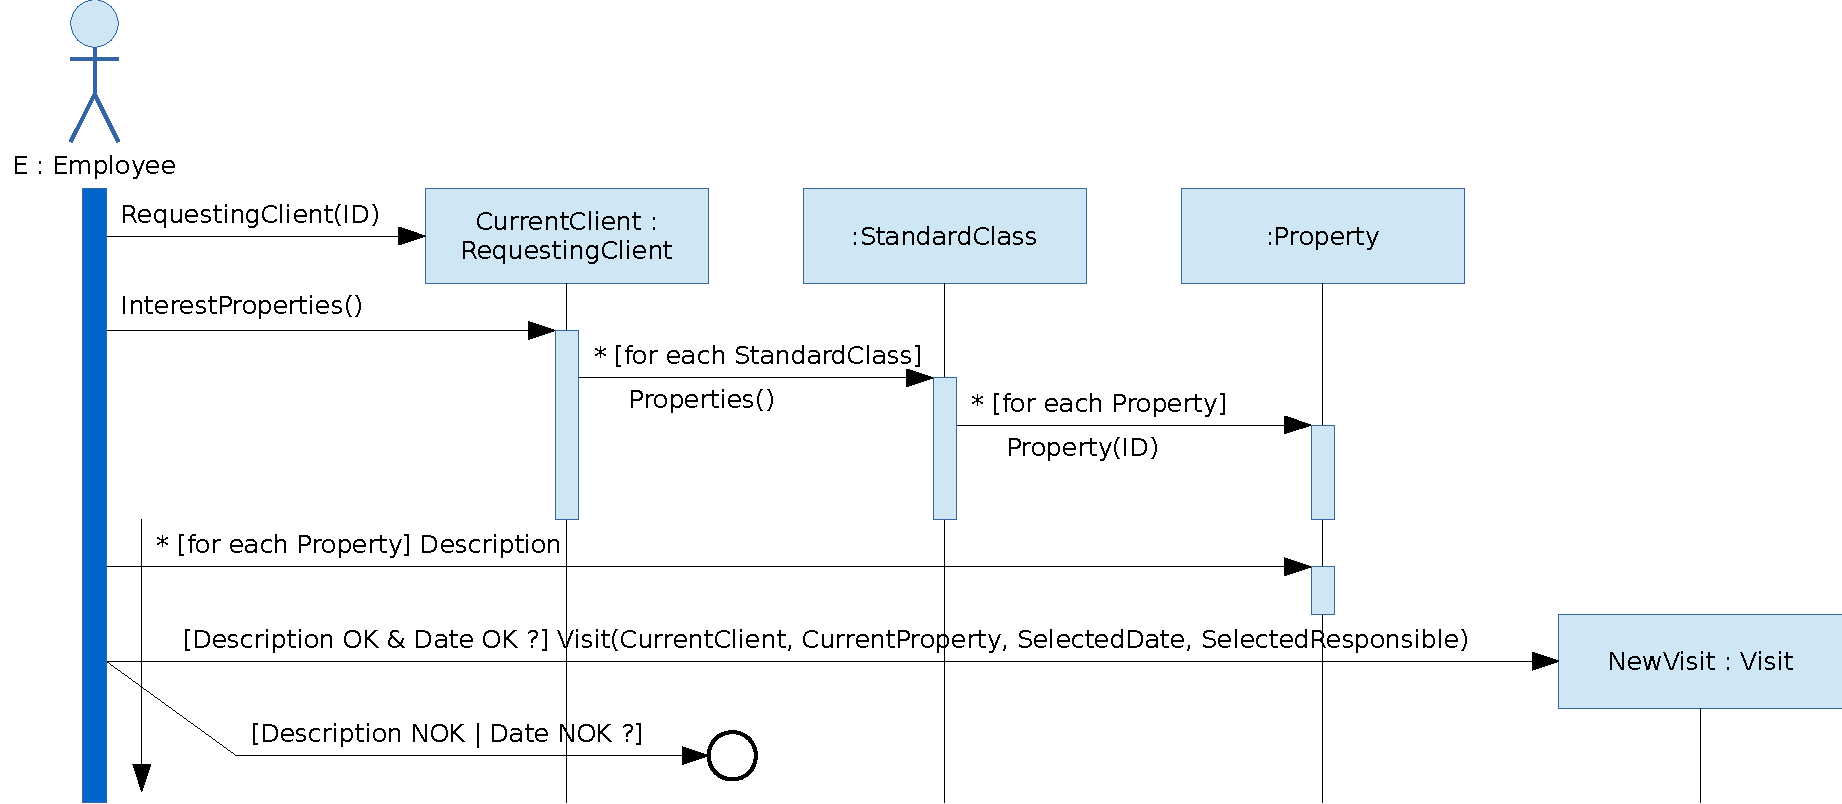
\includegraphics[scale=0.6,angle=90]{IMG/id}
  \caption{Diagramme de séquence}
  \label{img_id}
\end{figure}

La figure \refpage{img_id} illustre le diagramme de séquence du cas d'utilisation \selectedusecase{}.

\section{Rapport}

Ce diagramme est basé sur le diagramme d'activité du cas d'utilisation \selectedusecase{} et le diagramme de classes. Ce diagramme permettra d'avoir une vision sur la manière dont les classes interagissent entre elles pour ce cas d'utilisation ainsi que la manière dont il sera implémenté.

Au départ, si l'utilisateur du système a déjà traité des demandes pour le client, un objet de type \code{RequestingClient} existe déjà. Sinon, il faudra en créer un avec les données du client à traiter. Dans notre schéma il est appelé \code{CurrentClient}

Pour obtenir la liste des biens proposés au client, nous allons appeler la méthode \code{ProposedProperties()} de \code{CurrentClient}. Cette dernière va créer une série d'objets de type \code{ProposedProperty} qui correspondent aux différentes propriétés qui ont été proposées au client. La méthode va retourner cette liste.

Pour chacune des propriétés proposée et retournée par \code{ProposedProperties()}, l'utilisateur pourra consulter tous les attributs de la propriété via l'attribut \code{Property}. Ce dernier va retourner un objet de type \code{Property} Nous pourrons ensuite mettre à jour l'attribut \code{Interest} de l'objet de type \code{ProposedProperty} suivant les indications du client.

Pour obtenir la liste des biens retenus par le client, nous allons appeler la méthode \code{InterestProperties()} de \code{CurrentClient}. Cette dernière va créer une série d'objets de type \code{ProposedProperty} qui correspondent aux différentes propriétés qui ont été proposées au client et qui intéressent ce dernier, c'est à dire les objets de type \code{ProposedProperty} dont l'attribut \code{Interest} est à vrai. Pour chacun de ces objets, nous allons appeler l'attribut \code{Property} qui nous retournera un objet de type \code{Property} qui correspond à la propriété en elle-même. La liste de tous les objets de types \code{Property} sera renvoyé par \code{CurrentClient} à l'utilisateur.

Pour chaque propriété retournée par \code{InterestProperties()}, nous allons récupérer les visites déjà organisées grâce à la méthode \code{Visits()}. Cette dernière va retourner une liste d'objets de type \code{Visit}.

Une visite sera ensuite organisée ou non suivant les indications données par le client. Pour chacune des visite, nous allons créer un objet de type \code{Visit} en lui fournissant le client courant, la propriété concernée, la date choisie et le responsable de l'agence pour la visite. Ces informations seront alors enregistrées dans le système.